\begin{center}
  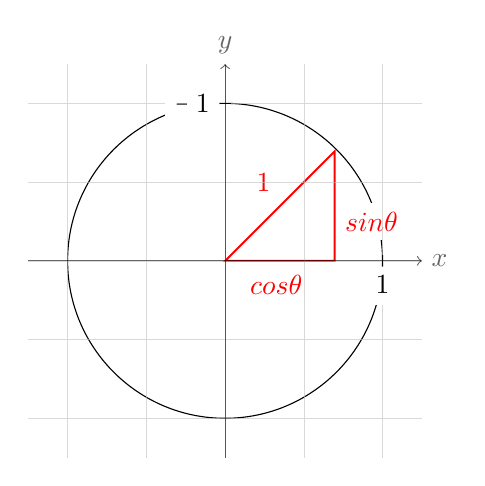
\begin{tikzpicture}
  %circle
   \draw[smooth, samples = 600] (0,0) circle (2)(1,1);
    		
    \draw[line width=0.25mm,red] (0,0) -- (1.39,1.39) -- (1.39,0)-- cycle;
    		\draw (0.7,1) node[left,red,fill=white] {$1$};
    		\draw (0.65,-0.3) node[red,fill=white] {$cos\theta$};
    		\draw (1.4,0.5) node[red,right,fill=white] {$sin\theta$};
    		
    \draw[opacity=0.6,lightgray,very thin,step=1cm](-2.5,-2.5) grid (2.5,2.5);
    \draw[->,opacity=0.6](-2.5,0) -- (2.5,0) node [right]{$x$};
    \foreach \x in {-1,...,1}
    \draw[xshift=2cm] (0,2pt) -- (0,-2pt) node[below,fill=white]{$\x$};
    \draw[->,opacity=0.6](0,-2.5) -- (0,2.5) node[above]{$y$};
    \foreach \y in {-1,...,1}
    \draw[yshift=2cm] (2pt,0) -- (-2pt,0) node[left,fill=white] {$\y$};
    	\end{tikzpicture}
    	\end{center}